\subsection{Bestimmung der Verdampfungswärme bei kleinem Druck}
\label{sec:bestimmungverdampfungswarme}
Die Verdampfungswärme kann als Porportionalitätsfaktor zwischen dem natürlichen Logarithmus des Druckes $P$ und der reziproken absoluten Temperatur $T$ aufgefasst werden. Die Wertepaare sind in Tabelle \ref{tab:druck-temperatur} dargestellt.
\begin{figure}
\captionof{table}{Wertepaare für die lineare Regression}	
	\centering
\input{testtabelle(besser).txt}
\label{tab:druck-temperatur}
\end{figure}

\begin{equation}
\ln(P) = - \frac{L}{\text{R}} \frac{1}{T} + \text{const.} = a \cdot \frac{1}{T} +b
\end{equation}
Lineare Regression nach Formeln aus Kaptel (VERWEIS) mittels Python liefert
\begin{equation}
a= \num{-4910(60)}  \text{Hässliche Einheit hinschreiben?}
\end{equation}
und damit eine Verdampfungswärme des Wassers von
\begin{equation}
L = - a \cdot R = \SI{40800(500)}{\joule\per\mol} 
\end{equation}
wobei $R$ die Gaskonstante mit \SI{8.314}{\joule\per\kelvin\per\mol} ist. \\
.


\begin{figure}[h!]
	\centering
	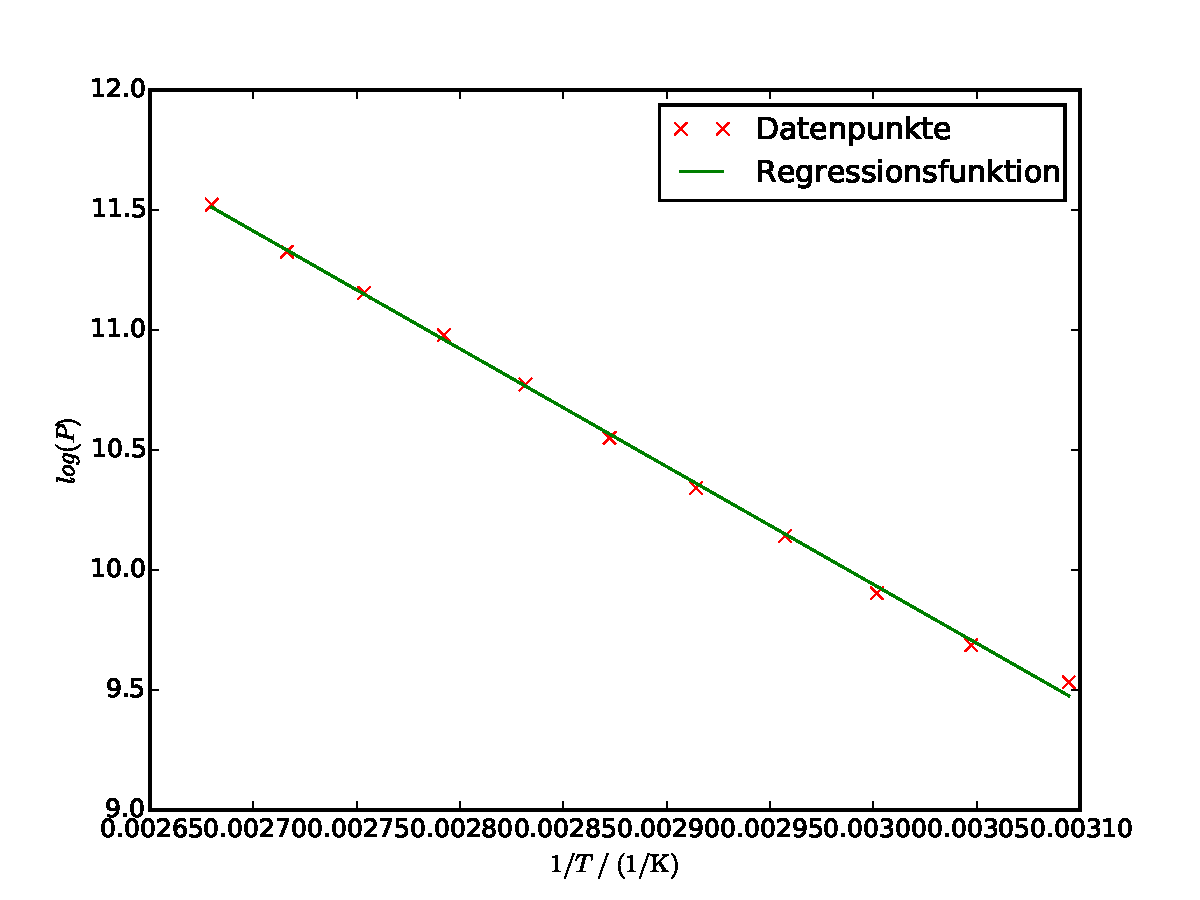
\includegraphics[width=0.95\textwidth]{L_kleiner_Druck.pdf}
	\caption{Logarithmus des Dampfdruckes gegen die reziproke absolute Temperatur}
	\label{fig:L_kleiner_Druck}
\end{figure}

\subsection{Unterscheidung zwischen äußerer und innerer Verdampfungswärme}
Die äußere Verdampfungswärme entspricht der Energie, die von System aufgewendet wird um zu expandieren. Diese Volumenarbeit ist bei einer Temperatur von  \SI{373}{\kelvin}
\begin{equation}
L_\text{a} = p \cdot V_\text{m} = R \cdot T = \SI{8.314}{\joule\per\kelvin\per\mol} \cdot  \SI{373}{\kelvin} \approx \SI{3101}{\joule\per\mol} \quad.
\end{equation}
Die innere Verdampfungswärme wird aufgebracht, um die wechselwirkenden Moleküle voneinander zu trennen. Da in Abschnitt \ref{sec:bestimmungverdampfungswarme} die gesamte Verdampfungswärme bestimmt wurde, entspricht die innere Verdampfungswärme gerade
\begin{equation}
L_\text{i} = L - L_{\text{a}} = \SI{40800}{\joule\per\mol} - \SI{3101}{\joule\per\mol} = \SI{37699}{\joule\per\mol} \quad.
\end{equation}
Die innere Verdampfungswärme ist dominierend. Bei Wasser beträgt der Wert der äußeren Verdampfungswärme unter Normaldruck nur etwa 10 \% des Wertes der Inneren.\footnote{siehe \url{http://portal.tugraz.at/portal/page/portal/Files/i5110/files/Lehre/Praktika/GP1/Vorbereitung/Verdampf_Gesamt.pdf}}




\subsection{Temperaturabhängigkeit der Verdampfungswärme bei hohem Druck}
Die Durckabhängigkeit der Verdampfungswärme ist nach Formel (VERWEIS) gegeben.

Zunächst wir der Druck als Funktion der Zeit dargestellt. Das Polynom dritten Grades wurde mit Hilfe von Python berechnet. Die hier angegebenen Werte für die Koeffizienten des Polynoms sind gerundet, obwohl mit exakten weiter gerechnet wurde.
\begin{equation}
P(T) = a \cdot T ^3 + b \cdot T^2 +c \cdot T + d
\end{equation}
\begin{align}
a &=0.626 \\
b &= 642 \\
c &= 221564 \\
d  &= 25769772
\end{align}
Die Ableitung des Druckes nach der Zeit ist
\begin{equation}
\frac{\text{d} P}{\text{d} T} = 3 \cdot a \cdot T^2 + 2 \cdot b \cdot T + c
\end{equation}
\begin{figure}[h!]
	\centering
	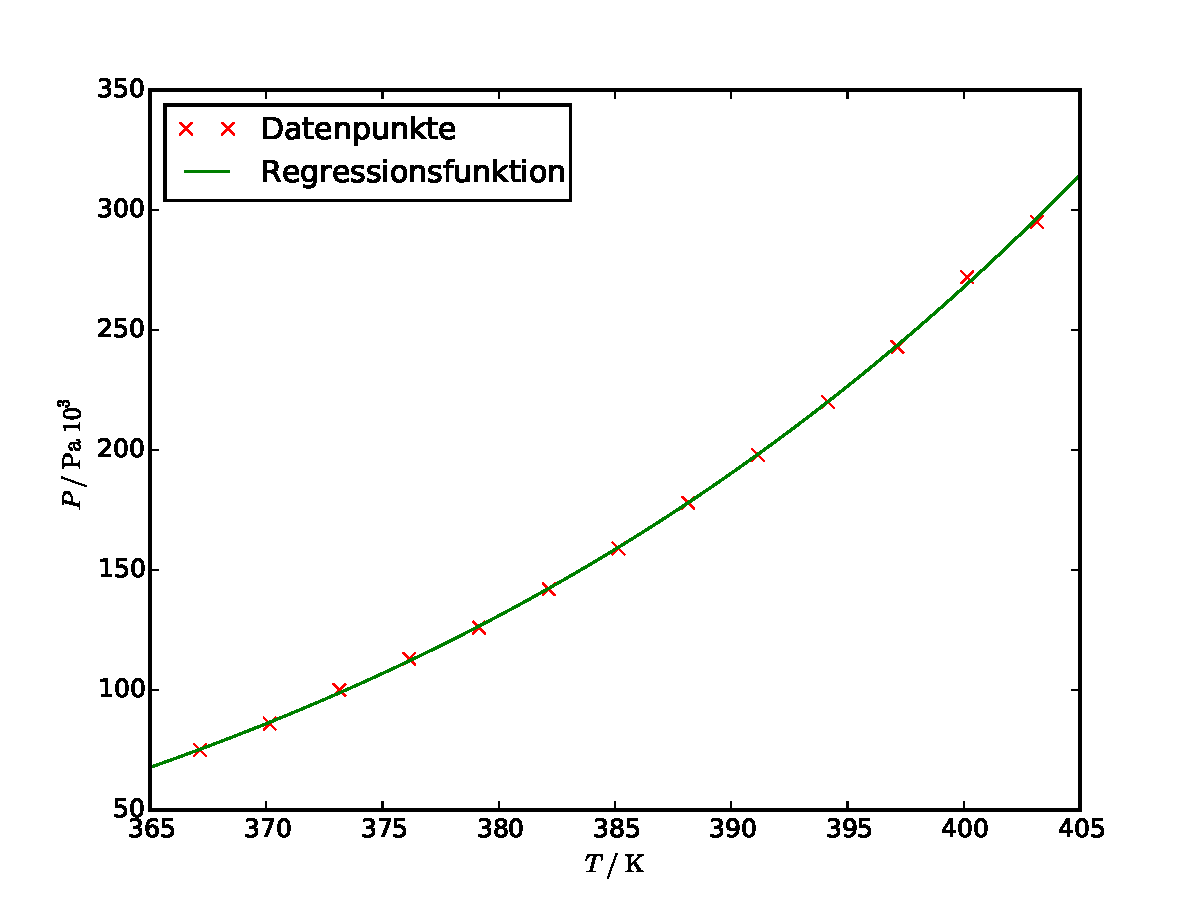
\includegraphics[width=0.95\textwidth]{Regerssionspolynom_P(t).pdf}
	\caption{Regressionspolynom dritten Grades des Druckes über die Temperatur}
	\label{fig:Regerssionspolynom_P(t)}
\end{figure}
\\

Die Volumenabhängigkeit von Temperatur und Druck kann hier nicht mehr vernachlässigt werden. Es gilt für das Volumen $V$
\begin{equation}
\left( P(T) + \frac{a_\text{W}}{V^2}\right) = R \cdot T \Leftrightarrow
V_{+,-} = \frac{R \cdot T \pm \sqrt{R^2 \cdot T^2 - 4 \cdot a_\text{W} \cdot P(T)}}{2 \cdot P(T)}
\end{equation}
Durch einsetzen der Ergebnisse ist ersichtlich, dass die Lösung $V_+$ unser Volumen widergibt. 
Bilder?!
\\
Nach dieser Vorarbeit ist
\begin{equation}
L(T) = V_+(P(T)) \cdot T \cdot \frac{\text{d} P}{\text{d} T} 
\end{equation}
und wurde in Abbildung \ref{fig:L_groser_druck_temperaturabhangig} über die Temperatur aufgetragen. Zusätzlich wurden Datenpunkte eingetragen, bei denen das Volumen durch die gemessenen Drücke, nicht das Regressionspolynom, berechnet wurde. 

Wertetabelle?!



\begin{figure}[h!]
	\centering
	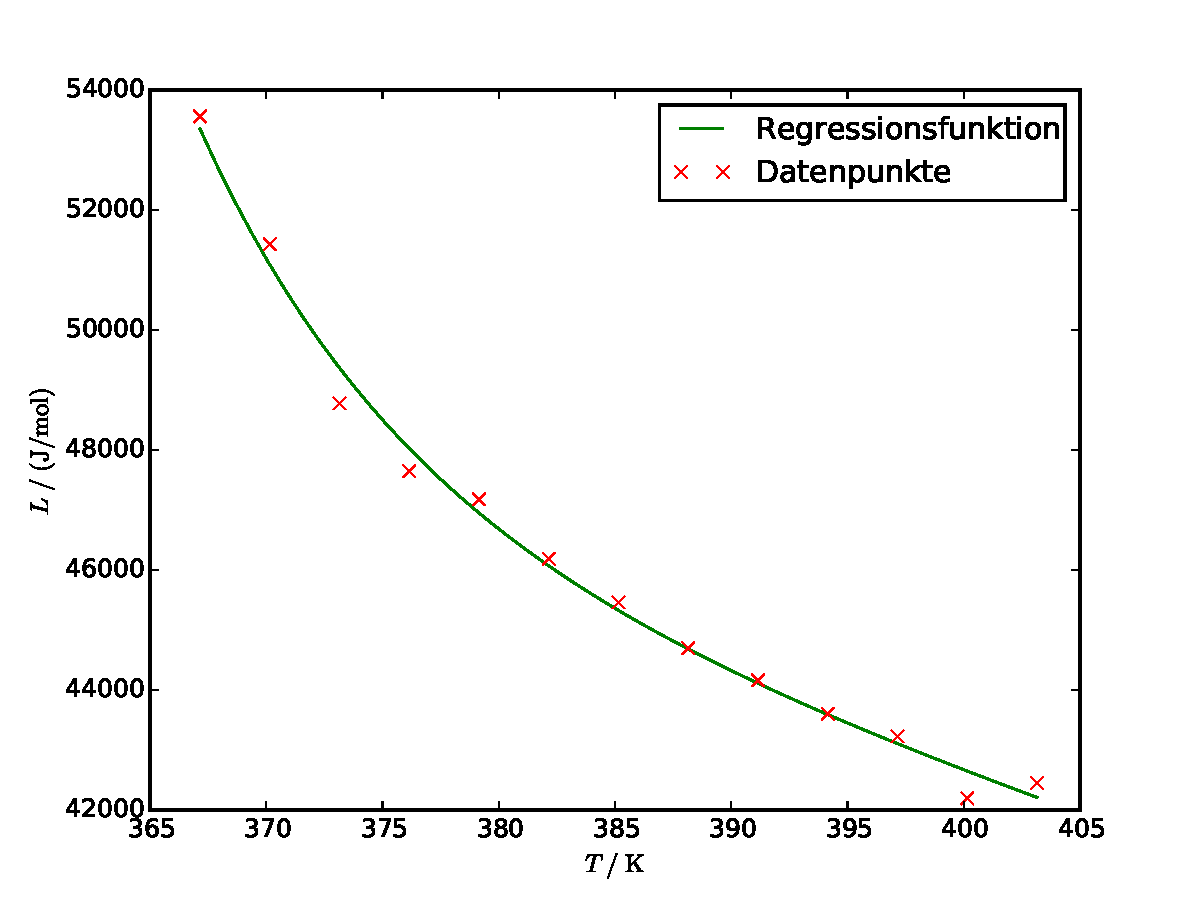
\includegraphics[width=0.95\textwidth]{L_groser_druck_temperaturabhangig.pdf}
	\caption{Verdampfungswärme in Abhängigkeit der Temperatur}
	\label{fig:L_groser_druck_temperaturabhangig}
\end{figure}





